\section{Evaluation}
\label{chap:evaluation}
Am Ende unserer Arbeit wurde uns ein Framework des SAFEST-Projekts zur Verfügung gestellt, dass die Möglichkeit bietet, verschiedene vorimplementierte Algorithmen mit einander zu vergleichen.\\
Nachdem wir unseren Algorithmus in das Framework integriert hatten, haben die folgenden Vergleiche mit einer vorimplementierten, Histogramm-basierten Lösung angestellt:
\begin{itemize}
	\item[a)] die vorimplementierte Lösung, die mit Histogrammen arbeitet
	\item[b)] unsere HMM-basierte Lösung mit generischen Werten für Initialwerte, Emission und Transition ohne Lernen
	\item[c)] unsere HMM-basierte Lösung mit generischen Werten für Initialwerte, Emission und Transition mit Lernen
	\item[d)] unsere HMM-basierte Lösung mit vorgelernten Werten
\end{itemize}
Weitere Vergleiche haben wir nicht angestellt, da das Histogramm-basierte Verfahren den anderen Verfahren entweder überlegen ist (OpenCV MOG und OpenCV MOG2) oder aber das Verfahren den Hintergrund hart auf bestimmte Videos kodiert (MEAN) und sehr unflexibel ist, sobald der Hintergrund nicht mehr uniform ist.\\
Das Ergebnis haben wir jeweils visualisiert, indem wir für jeden zu evaluierenden Algorithmus die Abweichung vom eigentlich erwarteten Wert visualisiert haben.
Ein optimal funktionierender Algorithmus würde also als Bild im Diagramm ohne Abweichungen die Nulllinie verdecken.\\
Die erwarteten Werte für diesen Vergleich sind uns seitens des SAFEST Projekts zur Verfüngung gestellt worden.
\subsection{Vergleich mit Histogramm-basierter Implementierung: Innenhof}
\label{sec:eval_innenhof}
\begin{figure}
	\centering
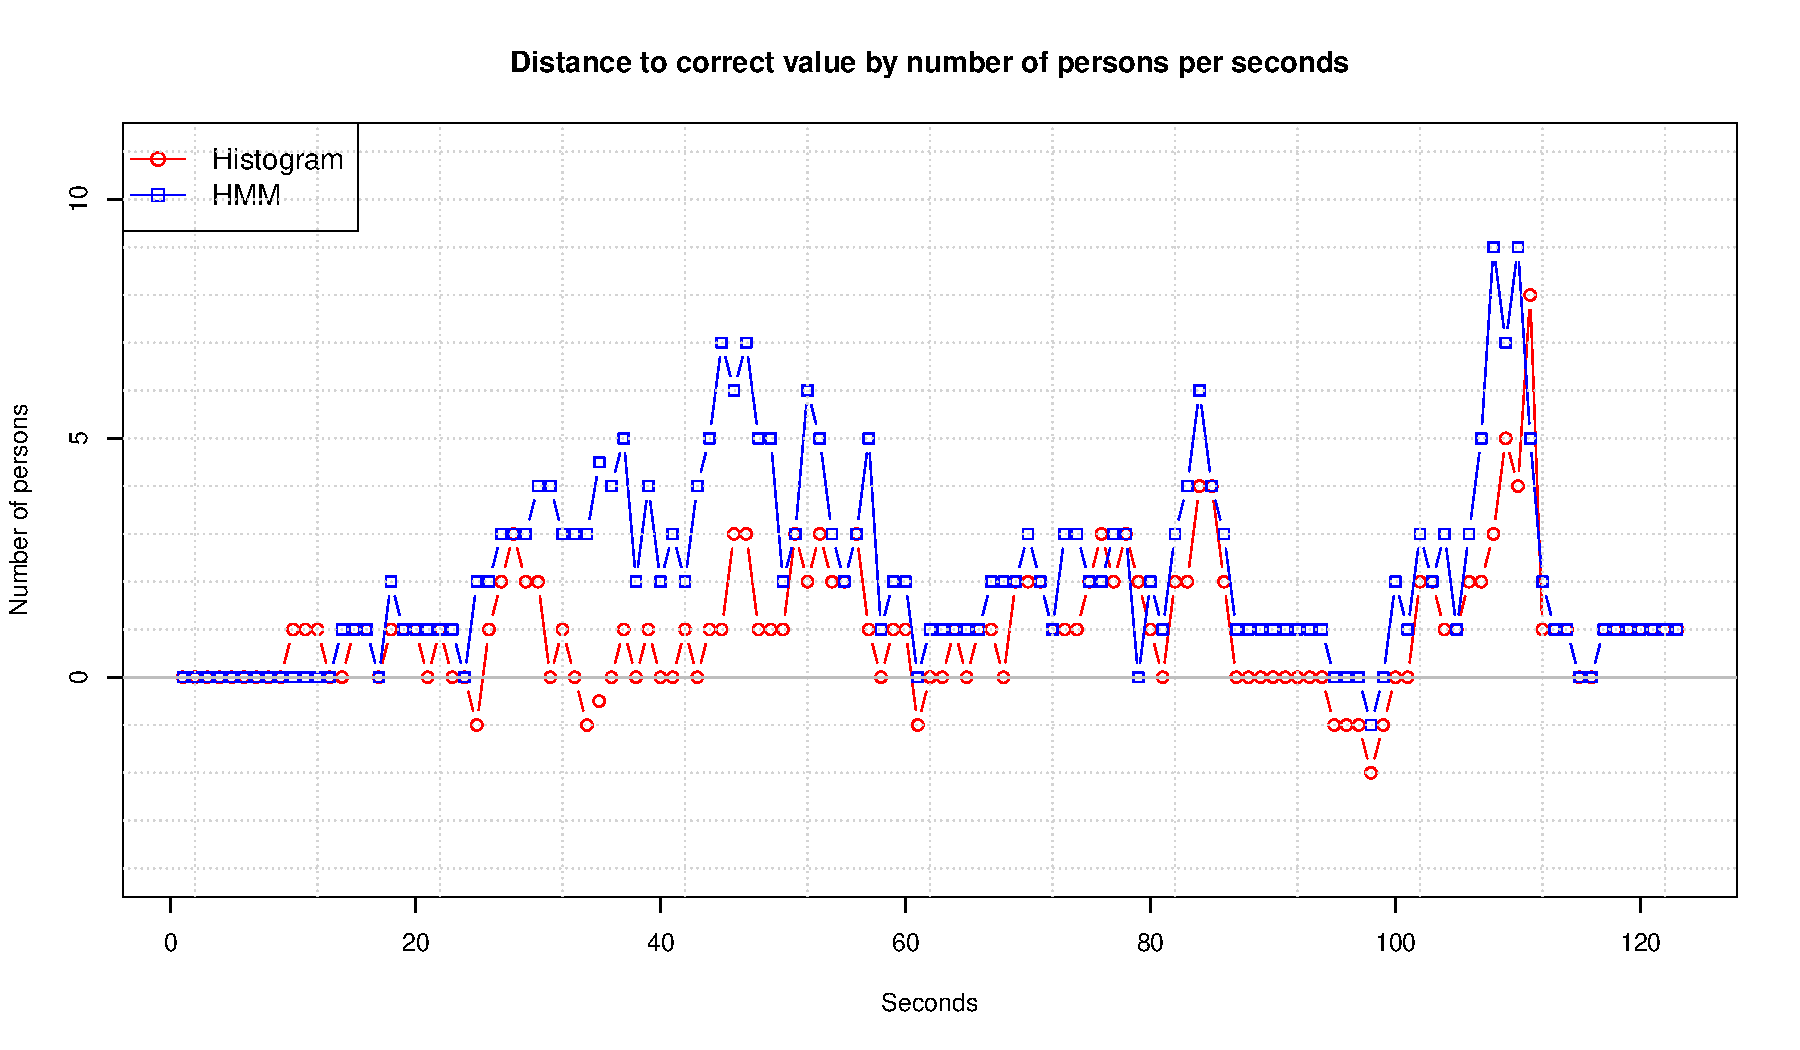
\includegraphics[width=1\textwidth]{bilder/safest_plot_tegel_7-55.pdf}
	\caption{Innenhof: Abweichung der getesteten Algorithmen vom echten Wert}
	\label{fig:Innenhof}
\end{figure}

\subsection{Vergleich mit Histogramm-basierter Implementierung: Eingang}
\label{sec:eval_eingang}
\begin{figure}
	\centering
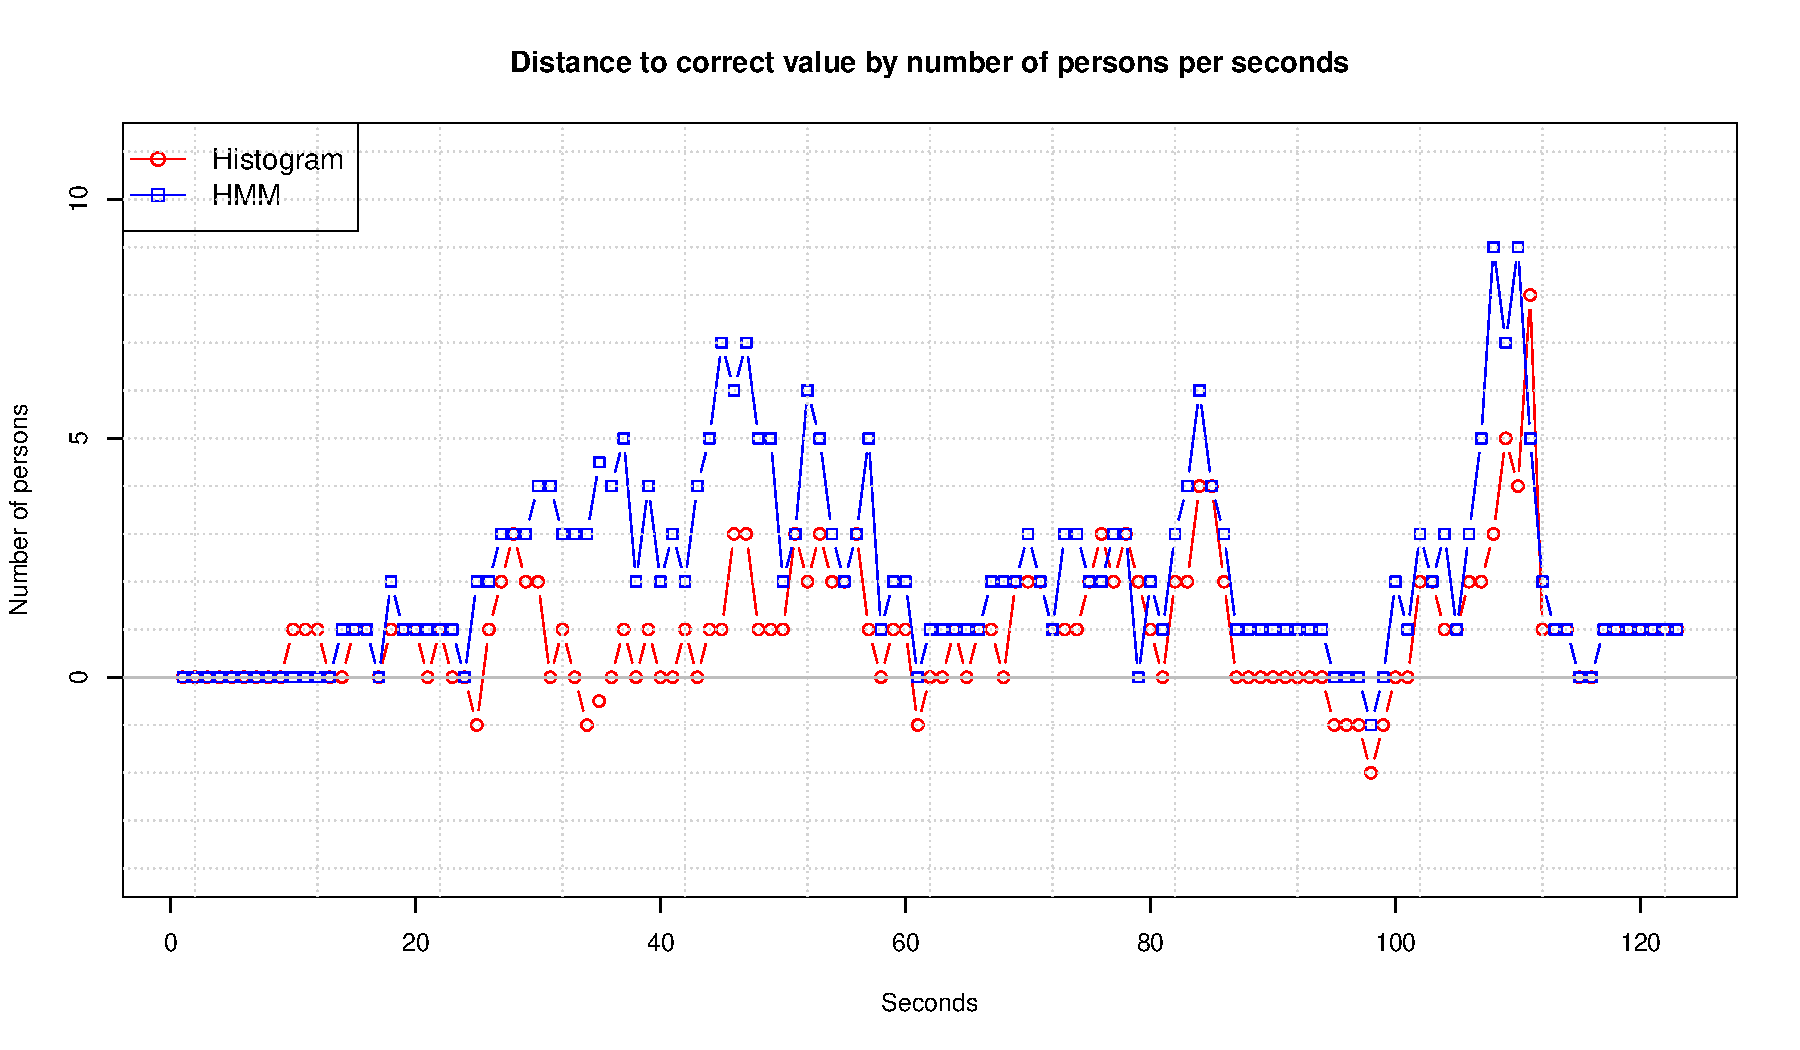
\includegraphics[width=1\textwidth]{bilder/safest_plot_tegel_7-55.pdf}
	\caption{Eingang: Abweichung der getesteten Algorithmen vom echten Wert}
	\label{fig:Eingang}
\end{figure}

\subsection{Vergleich mit Histogramm-basierter Implementierung: Tegel}
\label{sec:eval:tegel}
\begin{figure}
	\centering
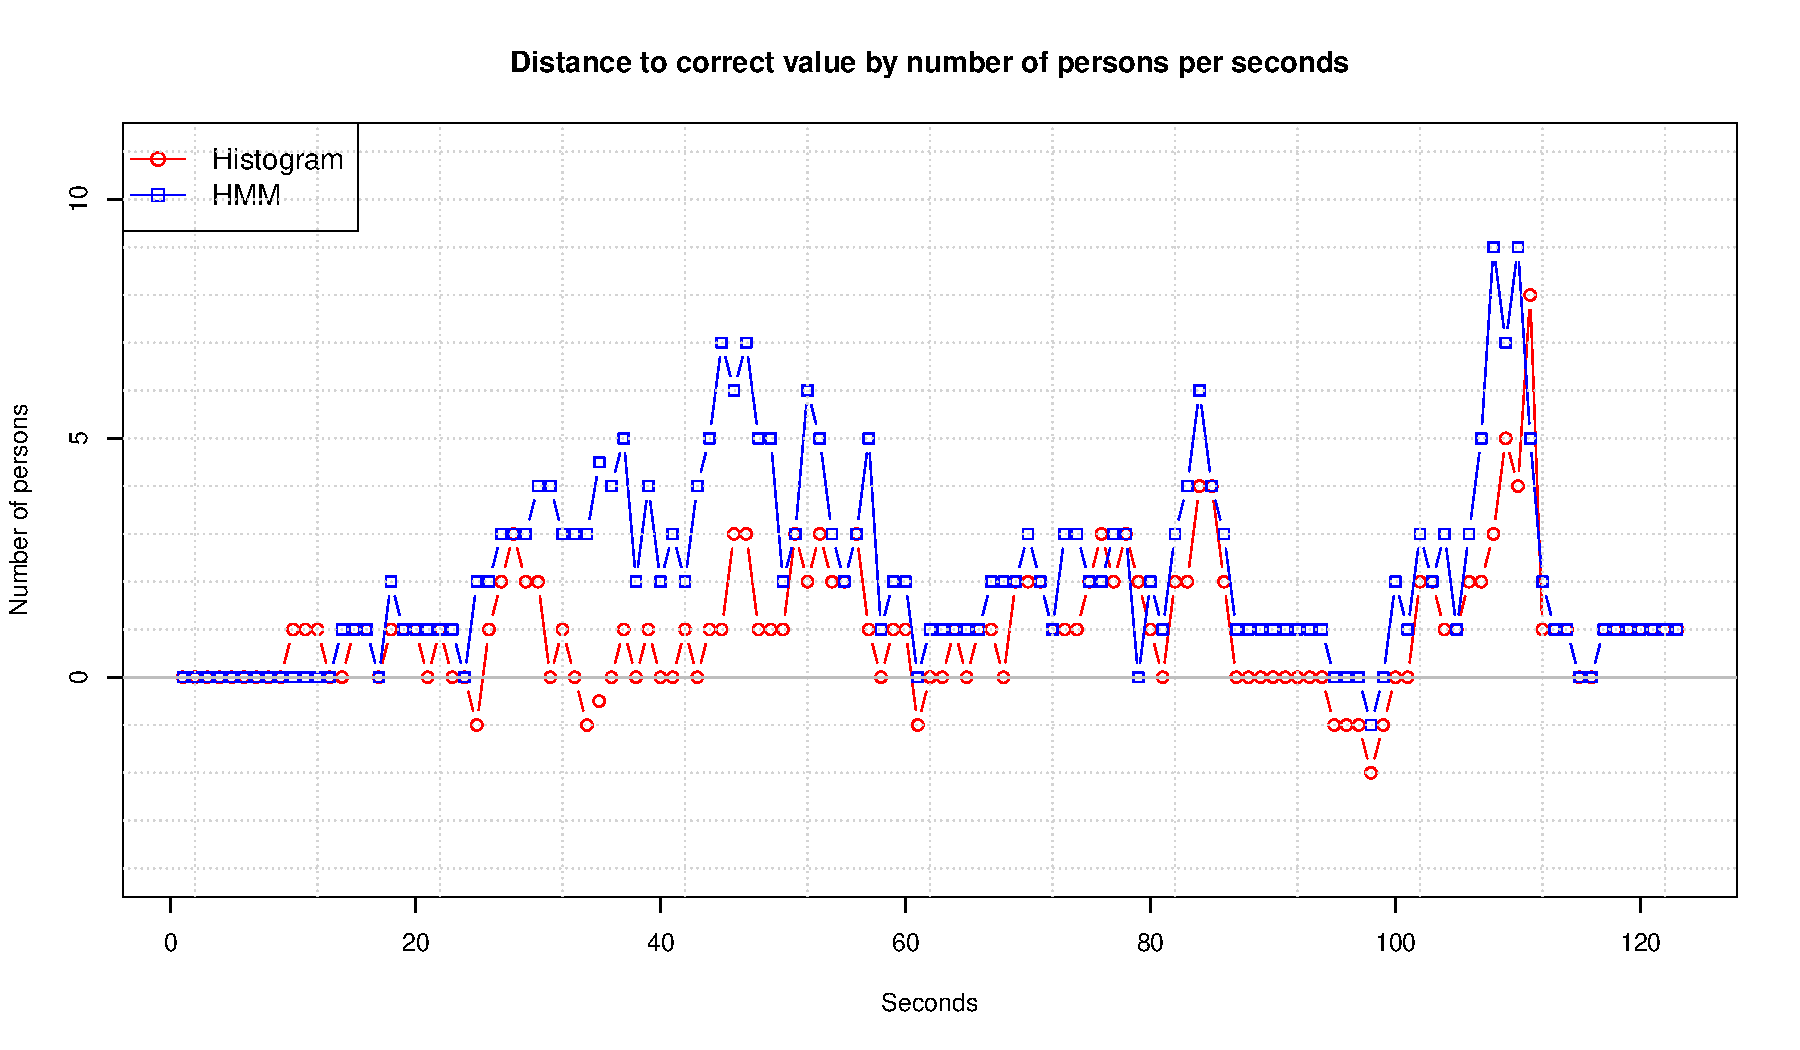
\includegraphics[width=1\textwidth]{bilder/safest_plot_tegel_7-55.pdf}
	\caption{Tegel: Abweichung der getesteten Algorithmen vom echten Wert, Video I}
	\label{fig:tegel_5-29}
\end{figure}

\begin{figure}
	\centering
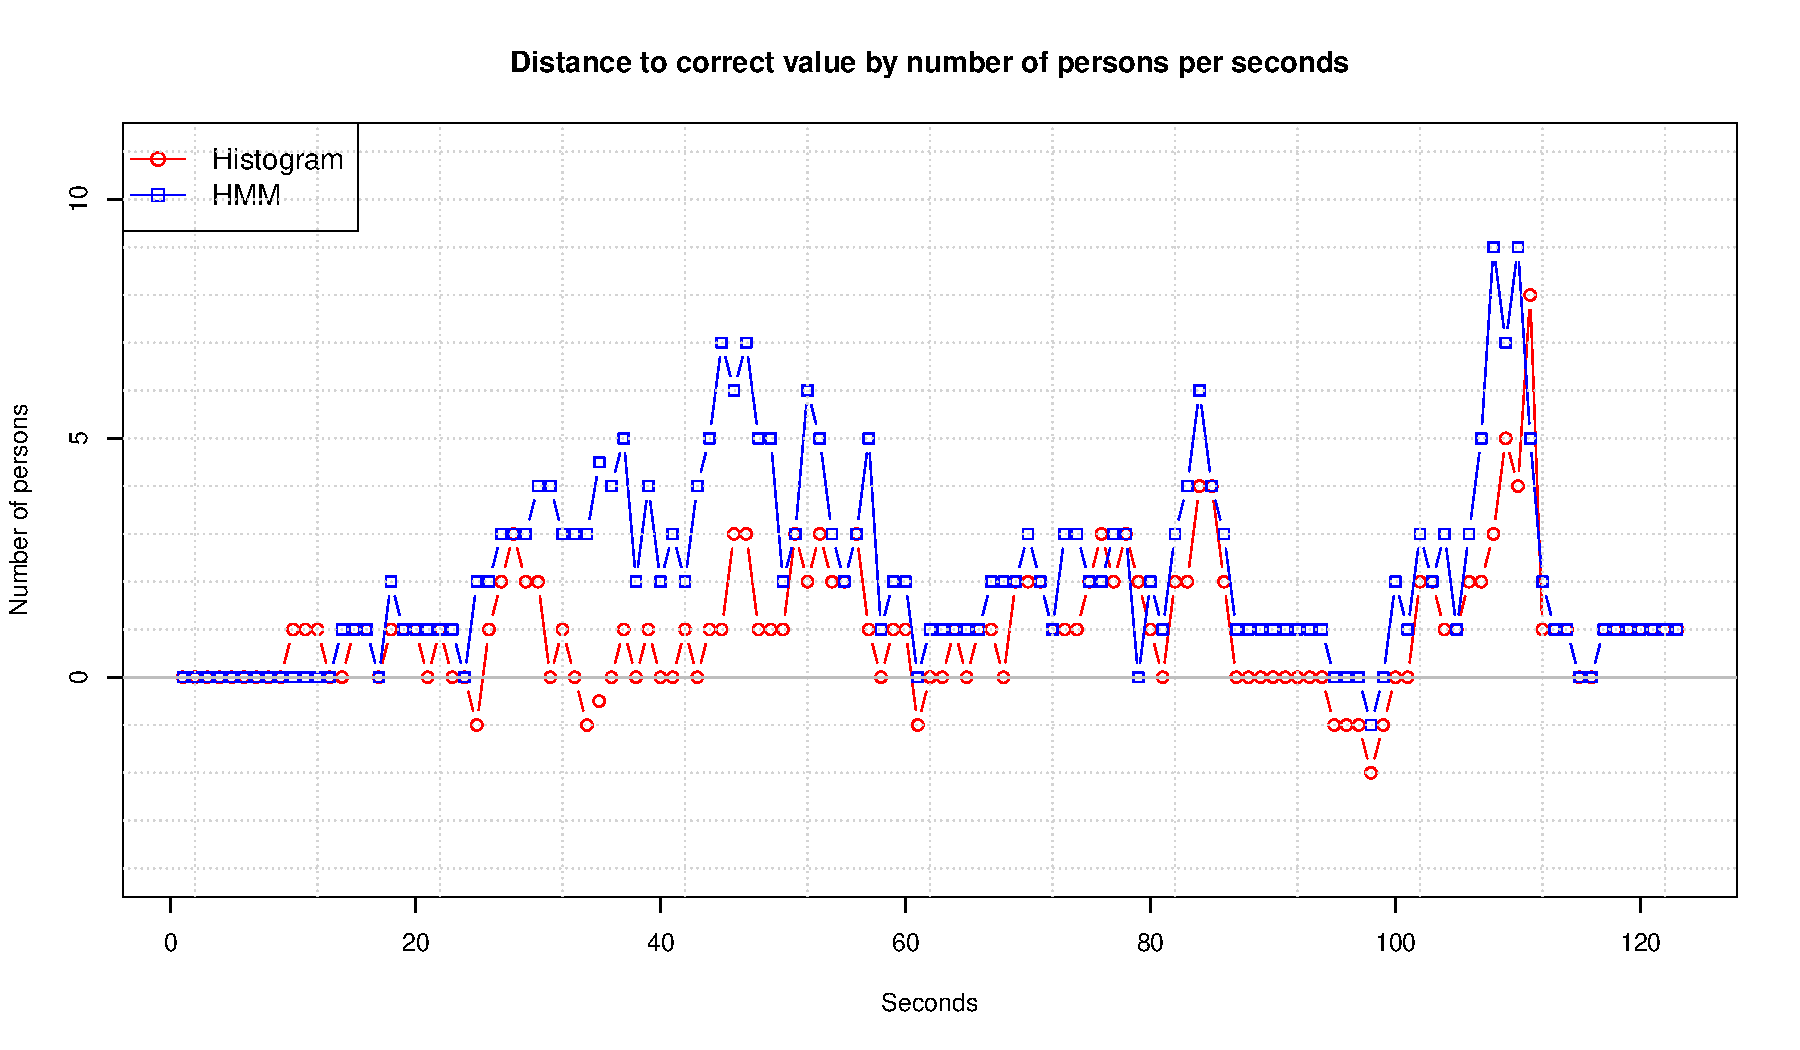
\includegraphics[width=1\textwidth]{bilder/safest_plot_tegel_7-55.pdf}
	\caption{Tegel: Abweichung der getesteten Algorithmen vom echten Wert Video II}
	\label{fig:tegel_7-55}
\end{figure}

\subsection{Diskussion}
\label{sec:diskussion}
 %bezug auf anforderungen nehmen, punkte erfüllt?
 %hmm topologie?
 %andere libs?
 %forward vs. viterbi
 %dynamische histrogramm/cluster grenzen für dc wert in zukunft?
 %viterbi/forawrd gibt zustand, man kann entweder gewichtestes würfeln oder aber deterministisch die wahrschienlichste beobachtung nehmen, was ist besser? -> test?
 %performance gewinn durch threading zusätzlich
